\section{Background}
\label{sec:background}
To begin we provide some background on genomics-based approaches to investigating cancers using next-generation sequencing (NGS) technology with its role and importance (Sec 2.1). Our key insight is that across a wide variety of computational genomics analysis flows, there are several common building blocks, which we call kernels as shown in Figure 1 with their software algorithms and characteristics. 
\begin{figure*}[htbp]
\centering
\includegraphics[scale=0.34]{fig/Kernels.pdf}
\caption{Overview of Genomic Kernels in the categories of genomic analysis flows.}
\label{fig:kernels}
\end{figure*}

\subsection{Clinical Cancer Research}
We first introduce three widely used genomic analytics pipelines. The rest of this section describes a typical software environment and then details the methodology that enables such analysis.

Genomic analytics is the process to synthesize genomic data into biological research or clinical knowledge including single-nucleotide variants (SNVs), INDELs, structural variants (SVs) and copy number variants (CNVs). Currently, the comprehensively used methods include Whole-Genome Sequencing (WGS), Whole-Exome Sequencing (WES), and targeted Gene Sequencing Panels (Panel). Table~\ref{tab:seqtypes} summarizes the comparison of these tools regarding data volume and requirement of data processing.

{\bf WGS.}~Whole-Genome Sequencing (WGS) delivers a comprehensive view of the entire genome. Through tumor-normal WGS, researchers can identify the comprehensive variants to a specific tumor sample. In other words, WGS is a universal and unbiased approach on condition that there are unlimited resources and time. Due to the base-pair resolution of an entire genome data analysis, its high computational cost is one of the major barriers to clinical applications. A WGS analysis pipeline needs several days that force us to reduce the execution time of a single job ({\em latency priority}). 

{\bf WES.}~Compared to WGS, Whole-Exome Sequencing (WES) is targeted to protein coding regions, so reads represent about $1\%$ of the genome. This reduces the cost to sequence a targeted region at a high depth and reduces storage and analysis costs. The much less cost allows researchers to increase the number of samples to be sequenced, enabling large population-based comparisons. Usually, in WES analysis there are multiple jobs each of which eeds several hours ({\em both latency and throughput priority}).

{\bf Panel.}~Targeted Gene Sequencing Panels are useful tools for analyzing specific mutations in a given sample. Since focused panels contain a select set of genes, Gene Panel also produces a smaller, more manageable data set, making analysis easier, compared to both WGS and WES. Usually, a typical Gene Panel Analytics Pipeline can be finished within one hour while there are more than tens of thousands pipeline in the same time ({\em throughput priority}).

\subsection{3D Memory}
3D stacked memory such as HMC (the focus of this paper) and HBM are promising in terms of PIM architectures~\cite{3Dstacking}. As shown in Figure~\ref{fig:arch_design}(b), 3D stacking involves a base logic die with layers of DRAM dies stacked on top of it. A memory cube can be partitioned into vertical slices called vaults, each with private vertical connections through all layers physically realized with TSVs. 3D stacked memory enables the stacking of base logic die and DRAM die. The base die of a memory cube is composed of several vertical slices, named as vaults. Memory banks on a given layer are partitioned into bank groups (usually one bank group per vault per layer), and each bank group shares the same TSVs allowing them to communicate among the vault layers. Intra-vault communication occurs through the TSVs, and inter-vault communication occurs through Network-on-Chip (NoC) routers. Considering a system composed of 16 8 GB HMCs as an example, conventional processors are still limited to 320 GB/s of memory bandwidth assuming that the CPU chip has the same number of off-chip links as that of an HMC. In contrast, PIM exposes 8 TB/s (= 16 × 512 GB/s) of aggregate internal bandwidth to the in-memory computation units. Taking genomic kernels as example, this paper try to answer three critical question when using PIM: (1) How to communicate between different memory partitions (i.e., vaults), (2) how to design an architecture to maximize the utilization of internal memory bandwidth, (3) how to map big data across different vaults.

\section{Workload Analysis Methodology}

\textbf{Simulation Configuration.}~The experiments have been done using SNIPER simulator~\cite{sniper}. Cache access timings for different cache capacities were extracted using CACTI~\cite{CACTI_5.3}. The baseline architecture is described in Table II. We marked the region of interest (ROI) in the application code. We ran the graph reading portion in the cache warm-up mode and, upon entering the ROI, collected statistics for 600 million instructions across all the cores.

\begin{table}[!htbp]
    \caption{Baseline architecture}
    \label{tab:1}
    \vspace{-12pt}
\renewcommand{\arraystretch}{1}
 \setlength{\tabcolsep}{2.5pt}
    \begin{center}
        \begin{tabular}{ | l | l | }
            \hline
            \multirow{4}{*}{\textbf{core}} & 4 cores, ROB = 128-entry, load queue = 48-entry, \\
           & store queue = 32-entry, reservation station entries = \\
           & 36, dispatch width = issue width = commit width = \\
           & 4, frequency = 2.66GHz\\
            \hline
            \multirow{4}{*}{\textbf{caches}} & 3-level hierarchy, inclusive at all levels, writeback, \\
           & LRU (Least Recently Used) replacement policy, data \\
           & and tags parallel access, 64B cacheline, separate L1 \\
           &  data and instruction caches\\
            \hline
            \multirow{2}{*}{\textbf{L1D cache}} & private, 32KB, 8-way set-associative, data access \\
           & time = 4 cycles, tag access time = 1 cycle \\
            \hline
            \multirow{2}{*}{\textbf{L2 cache}} & private, 256KB, 8-way set-associative, data access  \\
           & time = 8 cycles, tag access time = 3 cycles \\
            \hline
            \multirow{2}{*}{\textbf{L3 cache (LLC)}} & shared, 8MB, 16-way set-associative, data access \\
           & time = 30 cycles, tag access time = 10 cycles \\
            \hline
            \multirow{2}{*}{\textbf{DRAM}} & DDR3, device access latency = 45ns, queue delay \\
           & modeled\\
            \hline
        \end{tabular}        
    \end{center}
\end{table}

\textbf{Dataset.}~We used the following datasets from 1000 Genomes Projects in our experiments: 146.9Giga base-pair reads (500GB\footnote{The sequenced reads are stored as ASCII strings (roughly 100 characters each)}, NA12878) for WGS pipeline, 65GB file for WES, and 20GB file for Panel pipeline. The known variant database used for count covariates stage is dbsnp\_138.b37. For both WES and Panel we simulate the case of different samples by creating multiple parallel jobs.


\section{Analyzing and Mitigating Data Movement}
Our goal in this work is to (1) show genomic pipelines and kernels that can be used to build them (2) understand the data movement related bottlenecks in genomic kernels (3) comprehensively analyze the benefits that PIM can provide for such workloads, which includes reducing data movement, parallelism, shorter access latency.

\subsection{FM-index}
\subsubsection{Algorithm Description}
Full-text minute-space (FM) index~\cite{bwt} is the widely used kernel in many align tools~\cite{ahmed2016comparison}, which follows the seed-and-extend model. The seeding stage needs to \textbf{exactly} align seeds of the reads back to the reference genome without any gap as shown in Figure~\ref{fig:algo-fm}. An FM-index is created by first taking the Burrows-Wheeler transform (BWT) of the input text in the following steps. \circled{1} The genome string T is identified as "abracadabra\$", \circled{2} and The genome string is represented by the matrix M where each row is a rotation of the text, and the rows have been sorted lexicographically. \circled{3} The BWT of the genome string T = "abracadabra\$" is "ard\$rcaaaabb", which is the last column labeled \textbf{L} of matrix M. The data structure feature is that the i character occurrence of a character c in the last column has the same rank as the ith occurrence of c in the first column. Thus, searching the query seed is done by a last-to-first mapping with the fomula, which can be defined as LF(i) = C[L[i]] + Occ(L[i], i). The C[L[i]] represents the number of symbols in BWT that are lexicographically smaller than character a. Occ(L[i], i) is the number of occurrences of a in the BWT string of the reference genome based on current position i, C[L[i]].

\begin{figure}[htbp]
\centering
\includegraphics[scale=0.30]{fig/analysis/algo-fm.pdf}
\caption{An example of data structures in FM-index based mapping}
\label{fig:algo-fm}
\end{figure}

\subsubsection{Data Movement Analysis}
We first justify the selection of our target application, i.e. DNA seeding, for two reasons. First, DNA seeding dominates the computational expensive DNA alignment task (the end-to-end application), which contains both DNA seeding and DNA extension. Previous work~\cite{yuanrong} has shown memory system is certainly the bottleneck for DNA seeding, motivating our key idea of adopting the near-data processing architecture for the accelerator design. Our profiling results in Figure~\ref{fig:data-fm} quantitatively show the bottleneck. As Figure~\ref{fig:data-fm} shows, the DRAM access accounts for 60\% in the CPI stack analysis; the number of Load/Store instructions takes 43.4\% among total number of instructions in Figure~\ref{fig:data-fm}; The energy breakdown shows that 49.4\% of total energy consumption is consumed by the DRAM.
\begin{figure}[htbp]
\centering
\includegraphics[scale=0.44]{fig/analysis/data-fm.pdf}
\caption{Profiling the FM-index kernel in BWA-MEM with Sniper and configuration in Table II: (a) CPI stack; (b) Instruction statistics; (c) Energy breakdown.}
\label{fig:data-fm}
\end{figure}

%We conclude that the Occ4 function are responsible for a significant portion of the data movement that take place during seeding phase.

\subsubsection{Analysis of PIM Effectiveness}
In this section, we analyze the main reason for huge data movement and the suitability of PIM execution. For each base m, new values of sp and ep are computed by accessing two locations of the Occ structure. These locations depend on m and the current values of sp and ep. There is no defined pattern between successive values of sp and ep. Accessing the elements stored in the BWT index requires pointer-chasing and is also referred to as FM-index-search (FIS). FIS is intrinsically a sequential operation because of the data dependency to the next address, and also often accesses random addresses. Thus, architectural advances in modern processors (e.g., multiple cache hierarchies, MLP, and prefetching) provide limited performance improvement for this phase. In addition, while the computation for FIS is relatively simple as shown in~\cite{yuanrong}, the main-memory latency is critical to the overall performance.

The access location in the BWT table jumps irregularly with large strides. There seems to be little locality between consecutive access locations. The irregular memory access is the main reason for the high data movement. PIM will reduce huge data movement and short access latency. Furthermore, the behaviors of individual seeding tasks, i.e. the elemental task for parallel computing, are independent, PIM will provide high parallelism.

Previous work~\cite{yuanrong} shows that for FM-index search, only a few types of operations are dominative, e.g. memory copy operations, bitwise operations, and simple arithmetic operations like integer addition/subtraction and integer shifting. Many other operations are needless, such as floating-point operations, multiplication/division, vector and other complicated operations. These operations can be performed at high performance on PIM core or our customized PIM accelerator (see Section~\ref{sec:arch}). We detail the design of PIM accelerator and evaluate the energy efficiency and performance PIM accelerator for FM-index in Section~\ref{sec:arch}.

\subsection{Hash}
\subsubsection{Algorithm Description}
Hash is widely used in many alignment tools like SOAP~\cite{Wang:2012hw}, Smalt~\cite{SMALT}, and in the cleanner stage Markduplicate~\cite{li2009sequence}. Hash table stores the starting position of k-mers of the reference genome with the length of n. For each sequencing read, potentially matching segments in the reference genome are identified from seed matches in the index. Hash table is senstitive to the value of n and takes the s as the sampling frequency. s means the distance of the starting position of two consecutive genome seeds. However, with the larger length of n, the hash table size becomes larger. Compared to FM-index based mapper, the hash table based mappers are much slower and memory demanding. They are also more sensitive, more comprehensive and more robust to sequence
errors. Thus, hash table are more suitable when mapping reads to highly repetitive genomic regions where structural variants are more likely to occur~\cite{SMALT}. Hash operation is also used in a cleaner stage like Markduplicate. This application identifies duplicated reads, which either due to clonal duplication via PCR before sequencing, or due to optical duplication while on the sequencer. Since the MarkDuplicate in GATK is implemented with Java, we include samtools markdup kernel in our analysis.

\begin{figure}[htbp]
\centering
\includegraphics[scale=0.4]{fig/analysis/algo-hash.pdf}
\caption{An example of data structures in Hash Table based mapping}
\label{fig:algo-hash}
\end{figure}

\subsubsection{Data Movement Analysis}
As shown in Figure~\ref{fig:algo-hash}, the critical path in hash index lookups consists of an ALU-intensive key hashing followed by pointer chasing through a node list. Previous work~\cite{yuanrong} has shown the the bulk of the indexing time is spent on memory-intensive node list traversals. Our profiling results in Figure~\ref{fig:data-hash} quantitatively show the bottleneck. As we observe from Figure~\ref{fig:data-hash}, 71.5\% of the total system energy is spent on data movement generated by hash. The majority of the data movement comes from random memory accesses in both the build and probe phases, which diminish both performance and energy-efficiency. Due to the high amount of data movement, hash-based markdupliacte is a good candidate for PIM execution.
\begin{figure}[htbp]
\centering
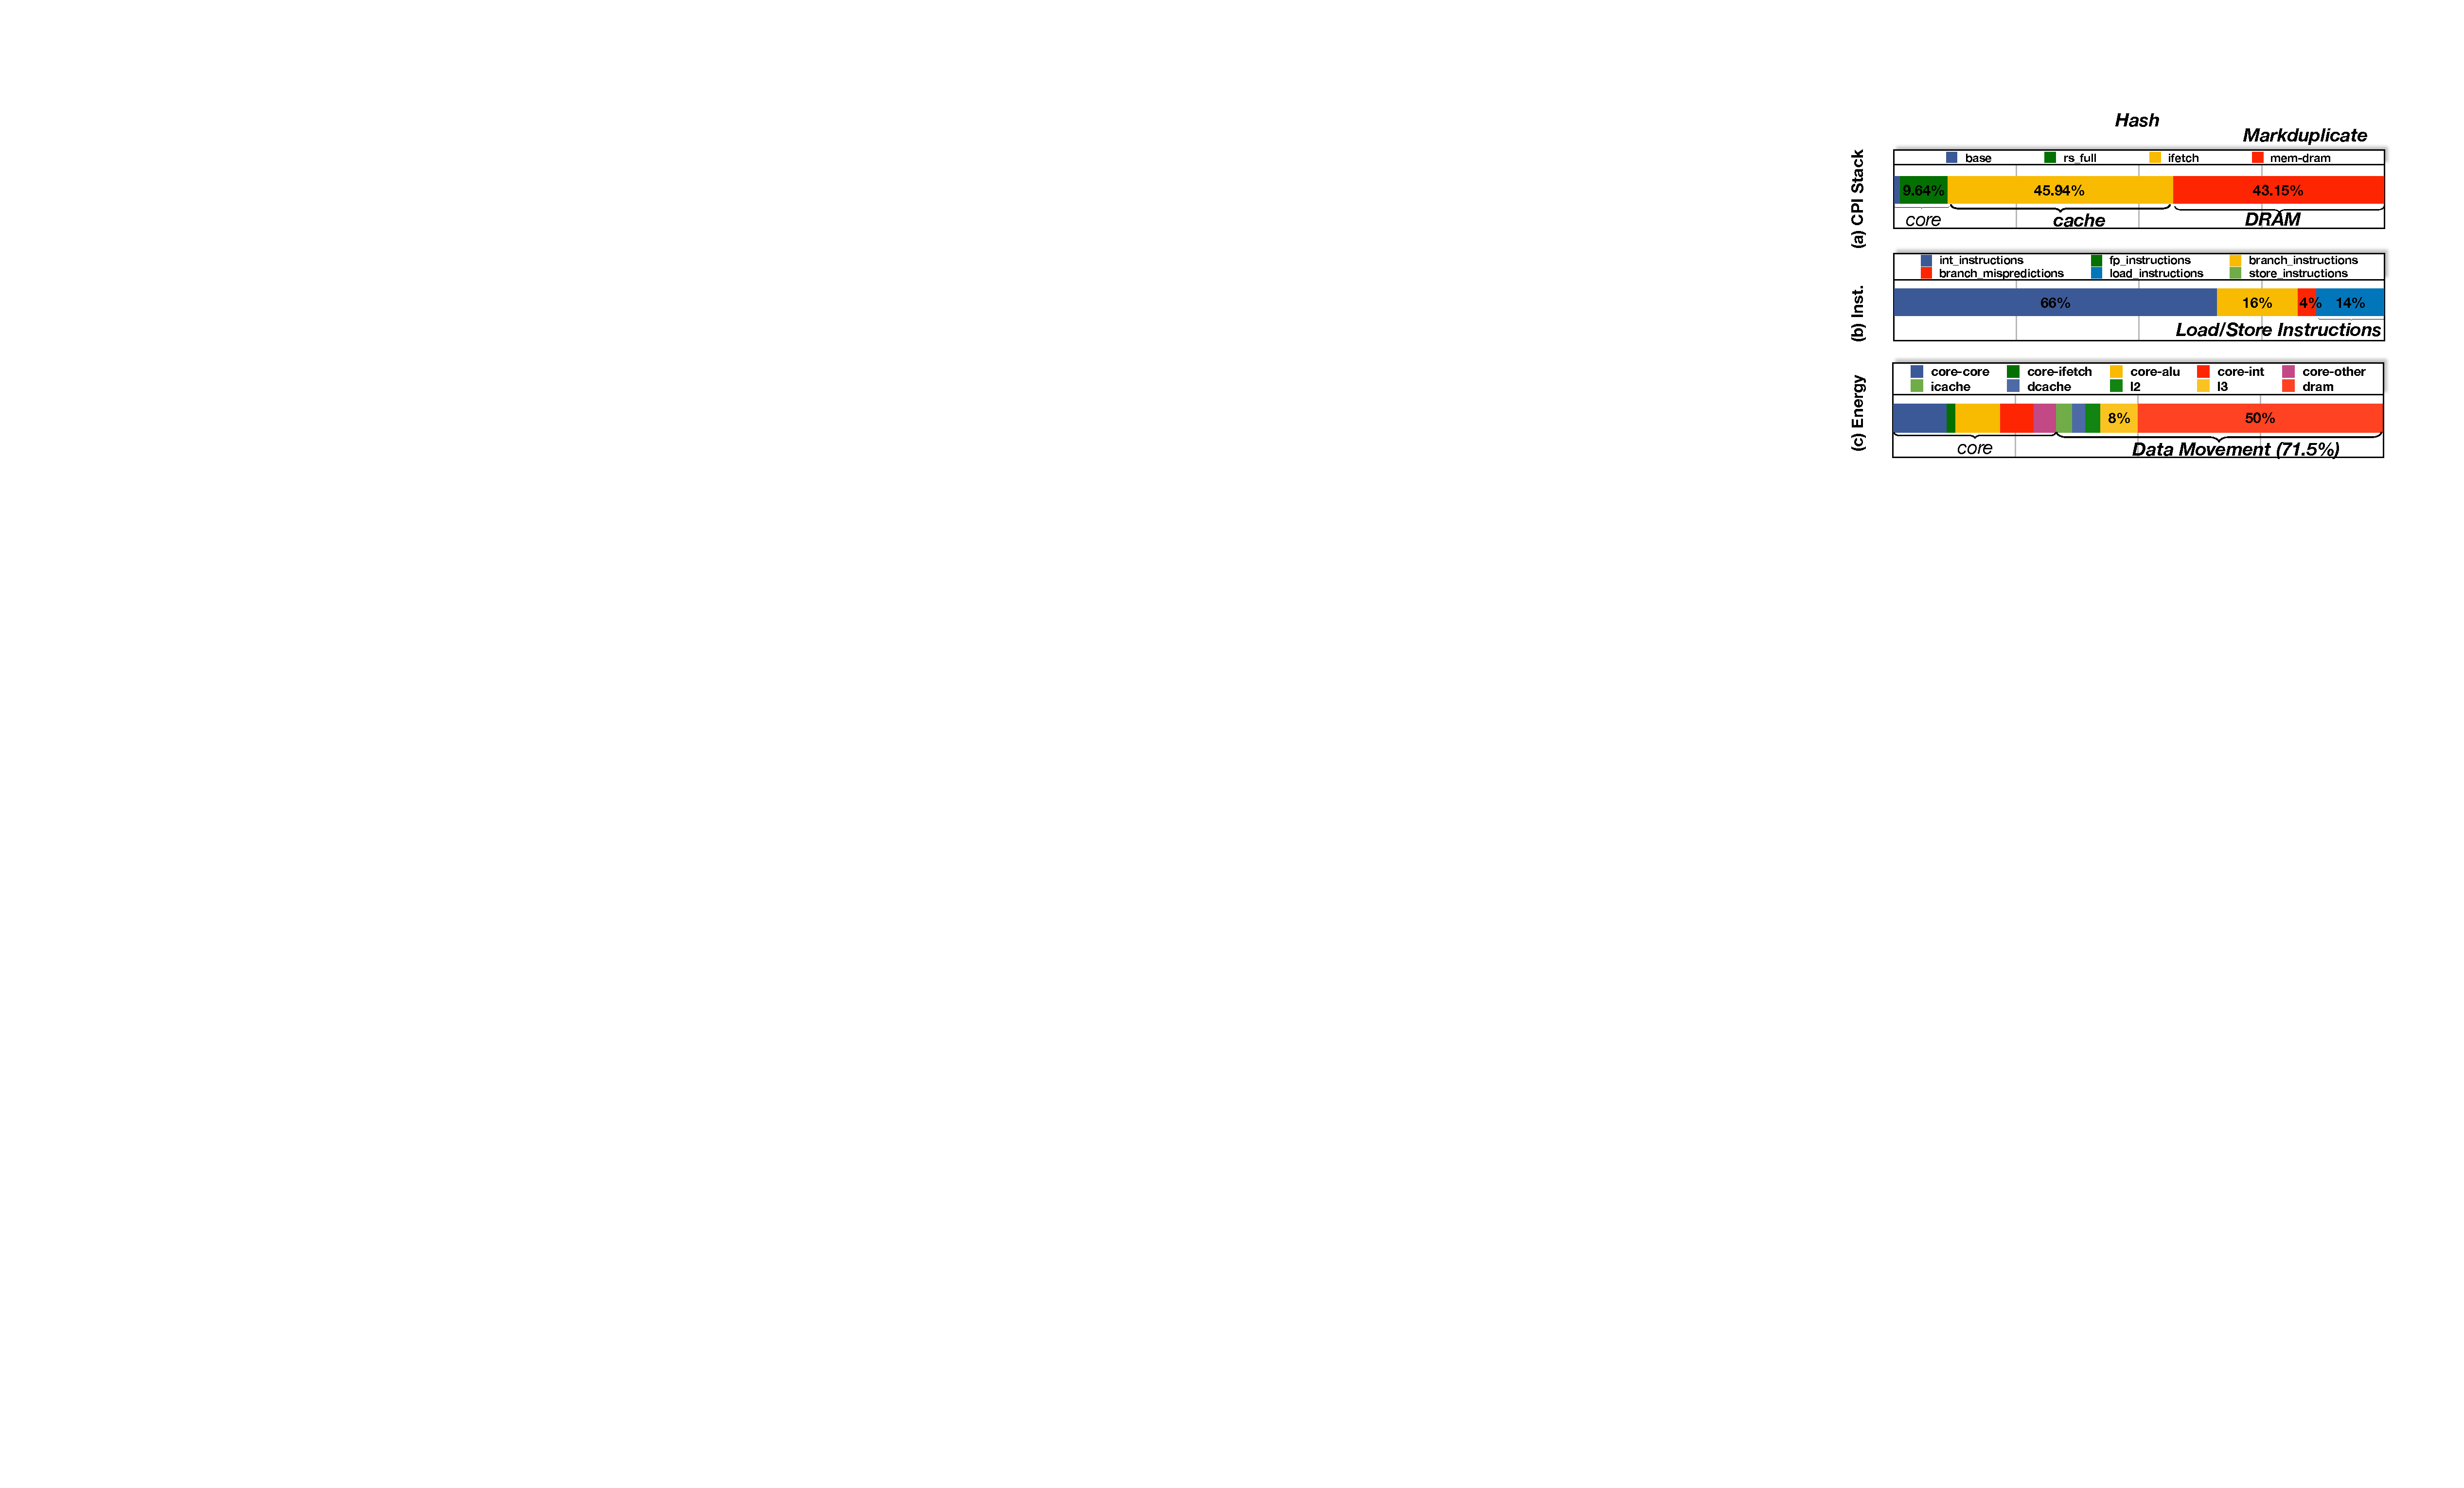
\includegraphics[scale=0.43]{fig/analysis/data-hash.pdf}
\caption{Profiling the Hash kernel in Markduplicate with Sniper and configuration in Table II: (a) CPI stack; (b) Instruction statistics; (c) Energy breakdown.}
\label{fig:data-hash}
\end{figure}

\subsubsection{Analysis of PIM Effectiveness}
Our analysis reveals that hash markduplicate requires only low-cost computations such as memcpy, simple arithmetic operations (e.g., addition and multiplication), and shift operations. These operations can be performed at high performance on our PIM core. Further, we make a critical observation that, because an indexing operation may touch millions of keys, enormous inter-key parallelism is offered/achieved. However, parallelism is constrained by hardware and physical limitations on conventional architecture.

%We conclude that the do\_hash() are responsible for a significant portion of the data movement that take place during seeding phase.

\subsection{Smith-Waterman}
\subsubsection{Algorithm Description}
As a famous Dynamic Programming (DP) algorithm, Smith-Waterman algorithm is the most widely used algorithm for several sequence mapping tools~\cite{bwt}, along with GATK Haplotype Caller~\cite{gatk-queue}. The input of this kernel is with numerous chains of seeds on short sequences with lengths rarely exceeding a few hundred bases. It compares a pair of sequences by computing a 2D scoring matrix for these two sequences to identify the most similar sub-sequences between them.

For a pair of nucleotides, there are three possibilities for the matching result, i.e., match, substitution, and insertion/deletion (gap). Element $H_{i,j}$ in this 2D matrix is calculated with equations below iteratively:

\begin{equation}
    E_{i,j} = max\{E_{i,j-1} - G_{ext}; H_{i,j-1} - G_{first}\}
\end{equation}

\begin{equation}
    F_{i,j} = max\{F_{i-1,j} - G_{ext}; H_{i-1,j} - G_{first}\}
\end{equation}

\begin{equation}
    H_{i,j} = max\{H_{i-1,j-1} + \sigma(a_i,b_j); E_{i,j}; F_{i,j}; 0\}
\end{equation}

where $\sigma(a_i,b_j)$ is the matching score between the $i$th element of sequence A and the $j$th element of sequence B. $G_{first}$ and $G_{ext}$ are the penalties for starting and extending a gap. Before computation, the matrix $H$, $E$, and $F$ are initialized with 0. The output is the best score S in H.

\subsubsection{Data Movement Analysis}
\begin{figure}[htbp]
\centering
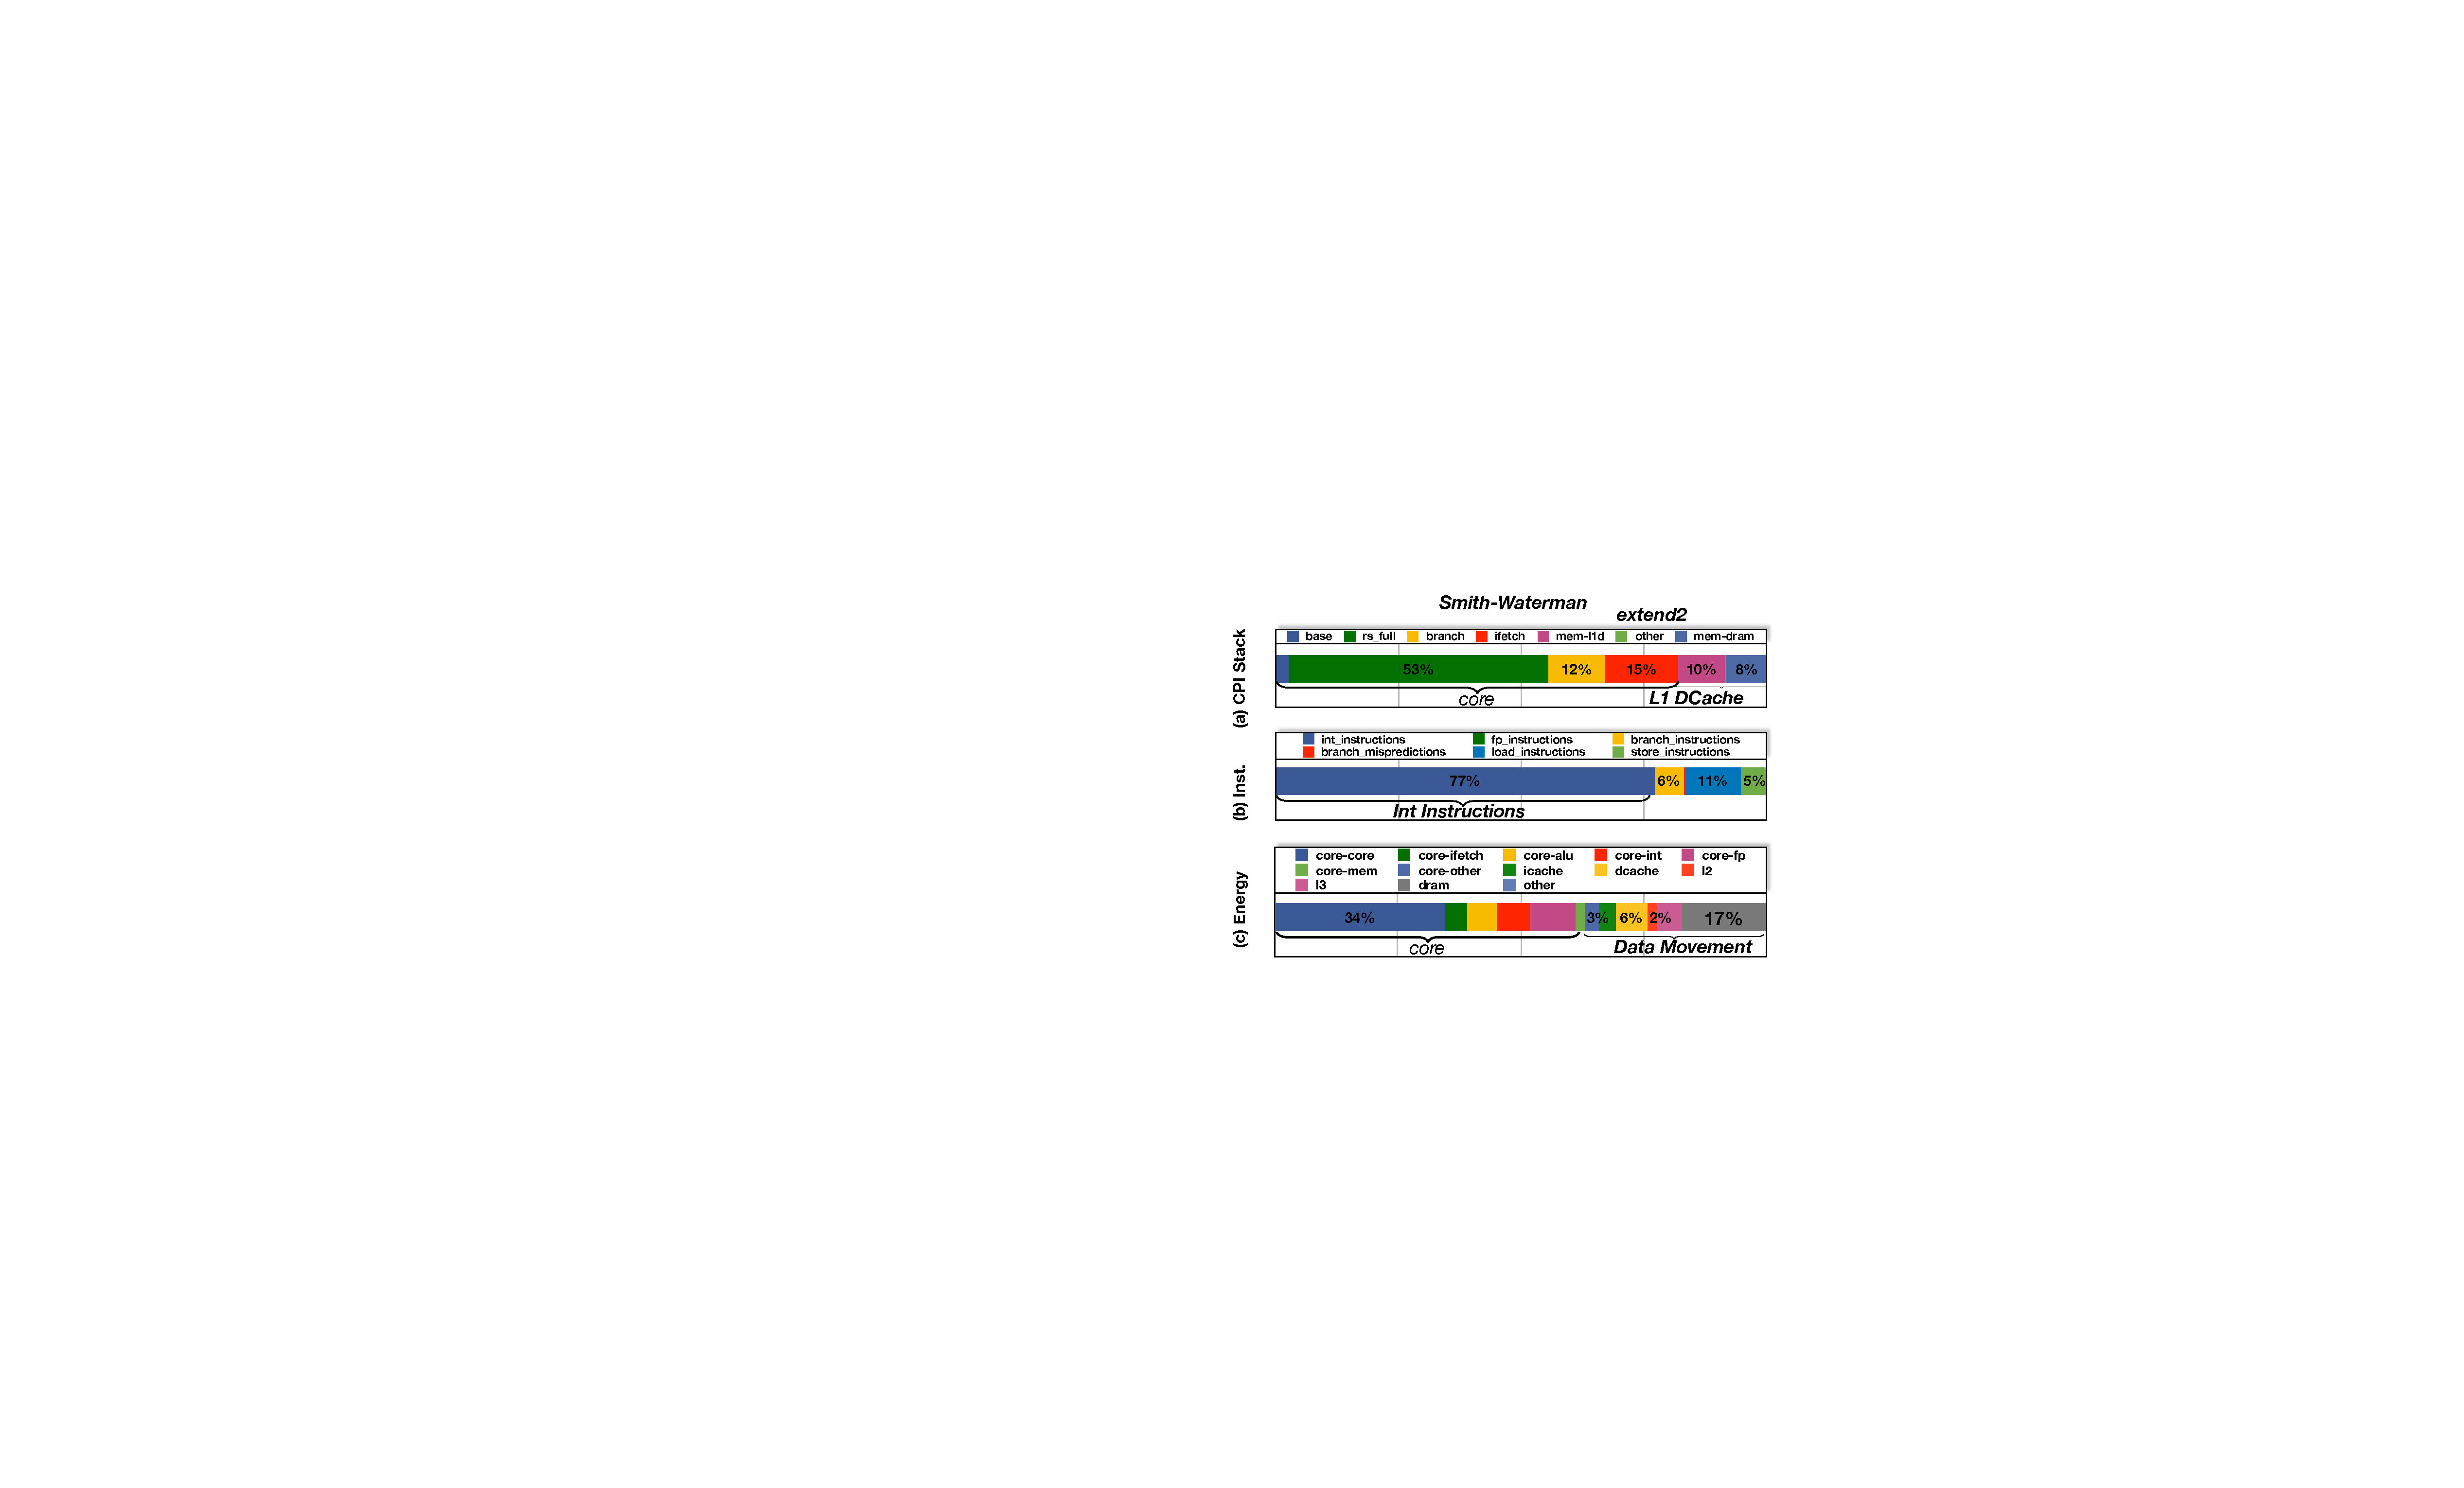
\includegraphics[scale=0.44]{fig/analysis/data-sw.pdf}
\caption{Profiling the Smith-Waterman kernel with Sniper and configuration in Table II: (a) CPI stack; (b) Instruction statistics; (c) Energy breakdown.}
\label{fig:data-sw}
\end{figure}

Figure~\ref{fig:data-sw} shows the characteristics of single-thread of Smith-Waterman. The DRAM access accounts for only 8\% in the CPI stack analysis. The number of Load/Store instructions takes 16\% among total number of instructions in Figure~\ref{fig:data-sw}(b). The energy breakdown in Figure~\ref{fig:data-sw}(c) shows that 32\% of total energy consumption is consumed by the data movement. Obviously, SW is a compute bound problem due to the following reasons: (1) Within a cell, cells of a matrix can be computed row by row. As the values in a row are only dependent on the same row and the one above it, only one row each of E, F and H needs to be maintained. (2) The input has a short sequence length, which ensures that E, F and H stay in the L1. We observed that the L1 miss rate is only about 0.20\%. However, the L2 and LLC miss rate are around 90.73\%, which means a miss in L1 will lead to a long latency memory access.

\begin{figure}[b]
\centering
\includegraphics[scale=0.55]{fig/analysis/data-sw-multi.pdf}
\caption{Profiling the multi-threaded Smith-Waterman kernel: CPI stack}
\label{fig:data-sw-multi}
\end{figure}

Since prior work showed that this kernel could simply be in the form of additional 56 cores, we take a look at the profile the SW kernel with 16 threads. As Figure~\ref{fig:data-sw-multi-energy} shows, the maximum memory access accounts for 68\% in the CPI stack analysis; The average DRAM access is over 49\% in the CPI stack. The energy breakdown in Figure~\ref{fig:data-sw-multi-energy} shows that 50.33\% of total energy consumption is consumed by the DRAM. Due to the high amount of data movement, we believe that when scaling to 56 cores, the data movement will be a huge bottleneck.

Usually, L1 data cache often has short latency comparable to ALU stalls. Profiling results show that the cache miss rate falls from 99.758\% to 82.170\% while the memory bandwidth utilization is only 19\%. L1 data cache stalls. We observed that relatively high LLC cache miss rates, which is more than 90.73\% in the multi-threaded SW kernel since the parallelization can not exploit data sharing in the shared cache so that multiple threads contend for the limited shared rooms.

\begin{figure}[htbp]
\centering
\includegraphics[scale=0.25]{fig/analysis/data-sw-multi-power.png}
\caption{Profiling the multi-threaded Smith-Waterman kernel with Energy breakdown.}
\label{fig:data-sw-multi-energy}
\end{figure}

\subsubsection{Inter- and Intra task Parallelism}
The scope for inter-task parallelism is obvious, as the pairwise alignments are independent of each other. With the intra-task, the calculation of cell (i, j) depends on three neighboring left cell (i, j-1), the above cell (i-1, j), and the diagonal above cell (i-1, j-1). The intra-task parallelsim lies in the anti-diagonal direction. Due to the short length of the anti-diagonals varies, the parallelism is limited. We then take a look at the computing operation of SW kernel. SW  only requires integer computation. The maximum possible score is directly proportional to the length of each sequence. For example, int8 operation can process 64 tasks in parallel.

\begin{table*}[t]
\centering
\caption{Computation and Memory Aceess Types of Genomic Kernels}
\fontsize{8}{10}\selectfont
\begin{tabular}{ |c|c|c|c|c| } 
\hline
\bf{Kernels} & \bf{Relevant Applications} & \bf{Execution Time} & \bf{Memory Access} & \bf{Example Operations} \\
\hline
FM-index Search & Seeding & Long & High & bit-wise operations \\
\hline
Smith-Waterman & Seed Extension, HaplotypeCaller & Medium & Medium & basic Integer arithmetic \\
\hline
Hash & Assembly, Markduplicate, HaplotypeCaller & Short & High & Shift operations, memcopy \\
\hline
Pair-HMM & HaplotypeCaller, Mutect2 & Medium & Medium & floating point operations (multiply and add) \\
\hline
\end{tabular}
\label{tab:time-breakdown}
\end{table*}

\subsection{Pair-HMM}
\subsubsection{Algorithm description}
As a variant of Smith-Waterman algorithm, Pair-HMM is commonly used in variant-calling. The hidden Markov model is used in Pair-HMM to generate a probability score for the alignment between candidate haplotypes (H) and read sequences (R). Similar to Smith-Waterman algorithm, for a pair of nucleotides, there are three possibilities for one pair of sequences, i.e., match, insertion, and deletion. The The key difference is that PairHMM uses floating point operations.

In Pair-HMM, three 2D matrices, i.e., match matrix $M$, insertion matrix $I$, and deletion matrix $D$, need to be computed. Elements $M_{i,j}$, $I_{i,j}$, and $D_{i,j}$ in those three matrices are calculated iteratively with equations:

\begin{equation}
    M_{i,j} = P_{i,j}(\alpha M_{i-1,j-1} + \beta I_{i-1,j-1} + \gamma D_{i-1,j-1})
\end{equation}

\begin{equation}
    I_{i,j} = \delta M_{i-1,j} + \epsilon I_{i-1,j}
\end{equation}

\begin{equation}
    D_{i,j} = \zeta M_{i,j-1} + \mu I_{i,j-1}
\end{equation}
where $\alpha$, $\beta$, $\gamma$, $\delta$, $\epsilon$, $\zeta$, $\mu$ are transition probabilities among different states. $P_{i,j}$ is the prior probability of emtting two characters $(a_i, b_j)$ in sequences $s_1$ and $s_2$. The similarity of the two sequences $s_1$ and $s_2$ are measured by the sum of all the cells in the last row of matrix $I$ and $D$.

The key difference is that PairHMM uses floating point operations. For this study, we used our optimized implementation that is also a part of the Genomics Kernel Library (GKL) by Intel.

\subsubsection{Data Movement Analysis}
Similar to SW, acceleration of PairHMM can exploit both intra-task parallelism and inter-task parallelism. Fot this study, we used the AVX optimized version of Pair-HMM used in GATK HaplotypeCaller and MuTect2. Figure~\ref{fig:data-pair} shows the DRAM access accounts for 54\% in the CPI stack analysis; The number of Load/Store instructions takes 25\% among total number of instructions in Figure~\ref{fig:data-pair}; The energy breakdown in Figure~\ref{fig:data-pair} shows that 53.62\% of total energy consumption is consumed by the data movement. Since PairHMM has very similar characteristics to SW, we do not make deeper analysis into PairHMM. 

\begin{figure}[htbp]
\centering
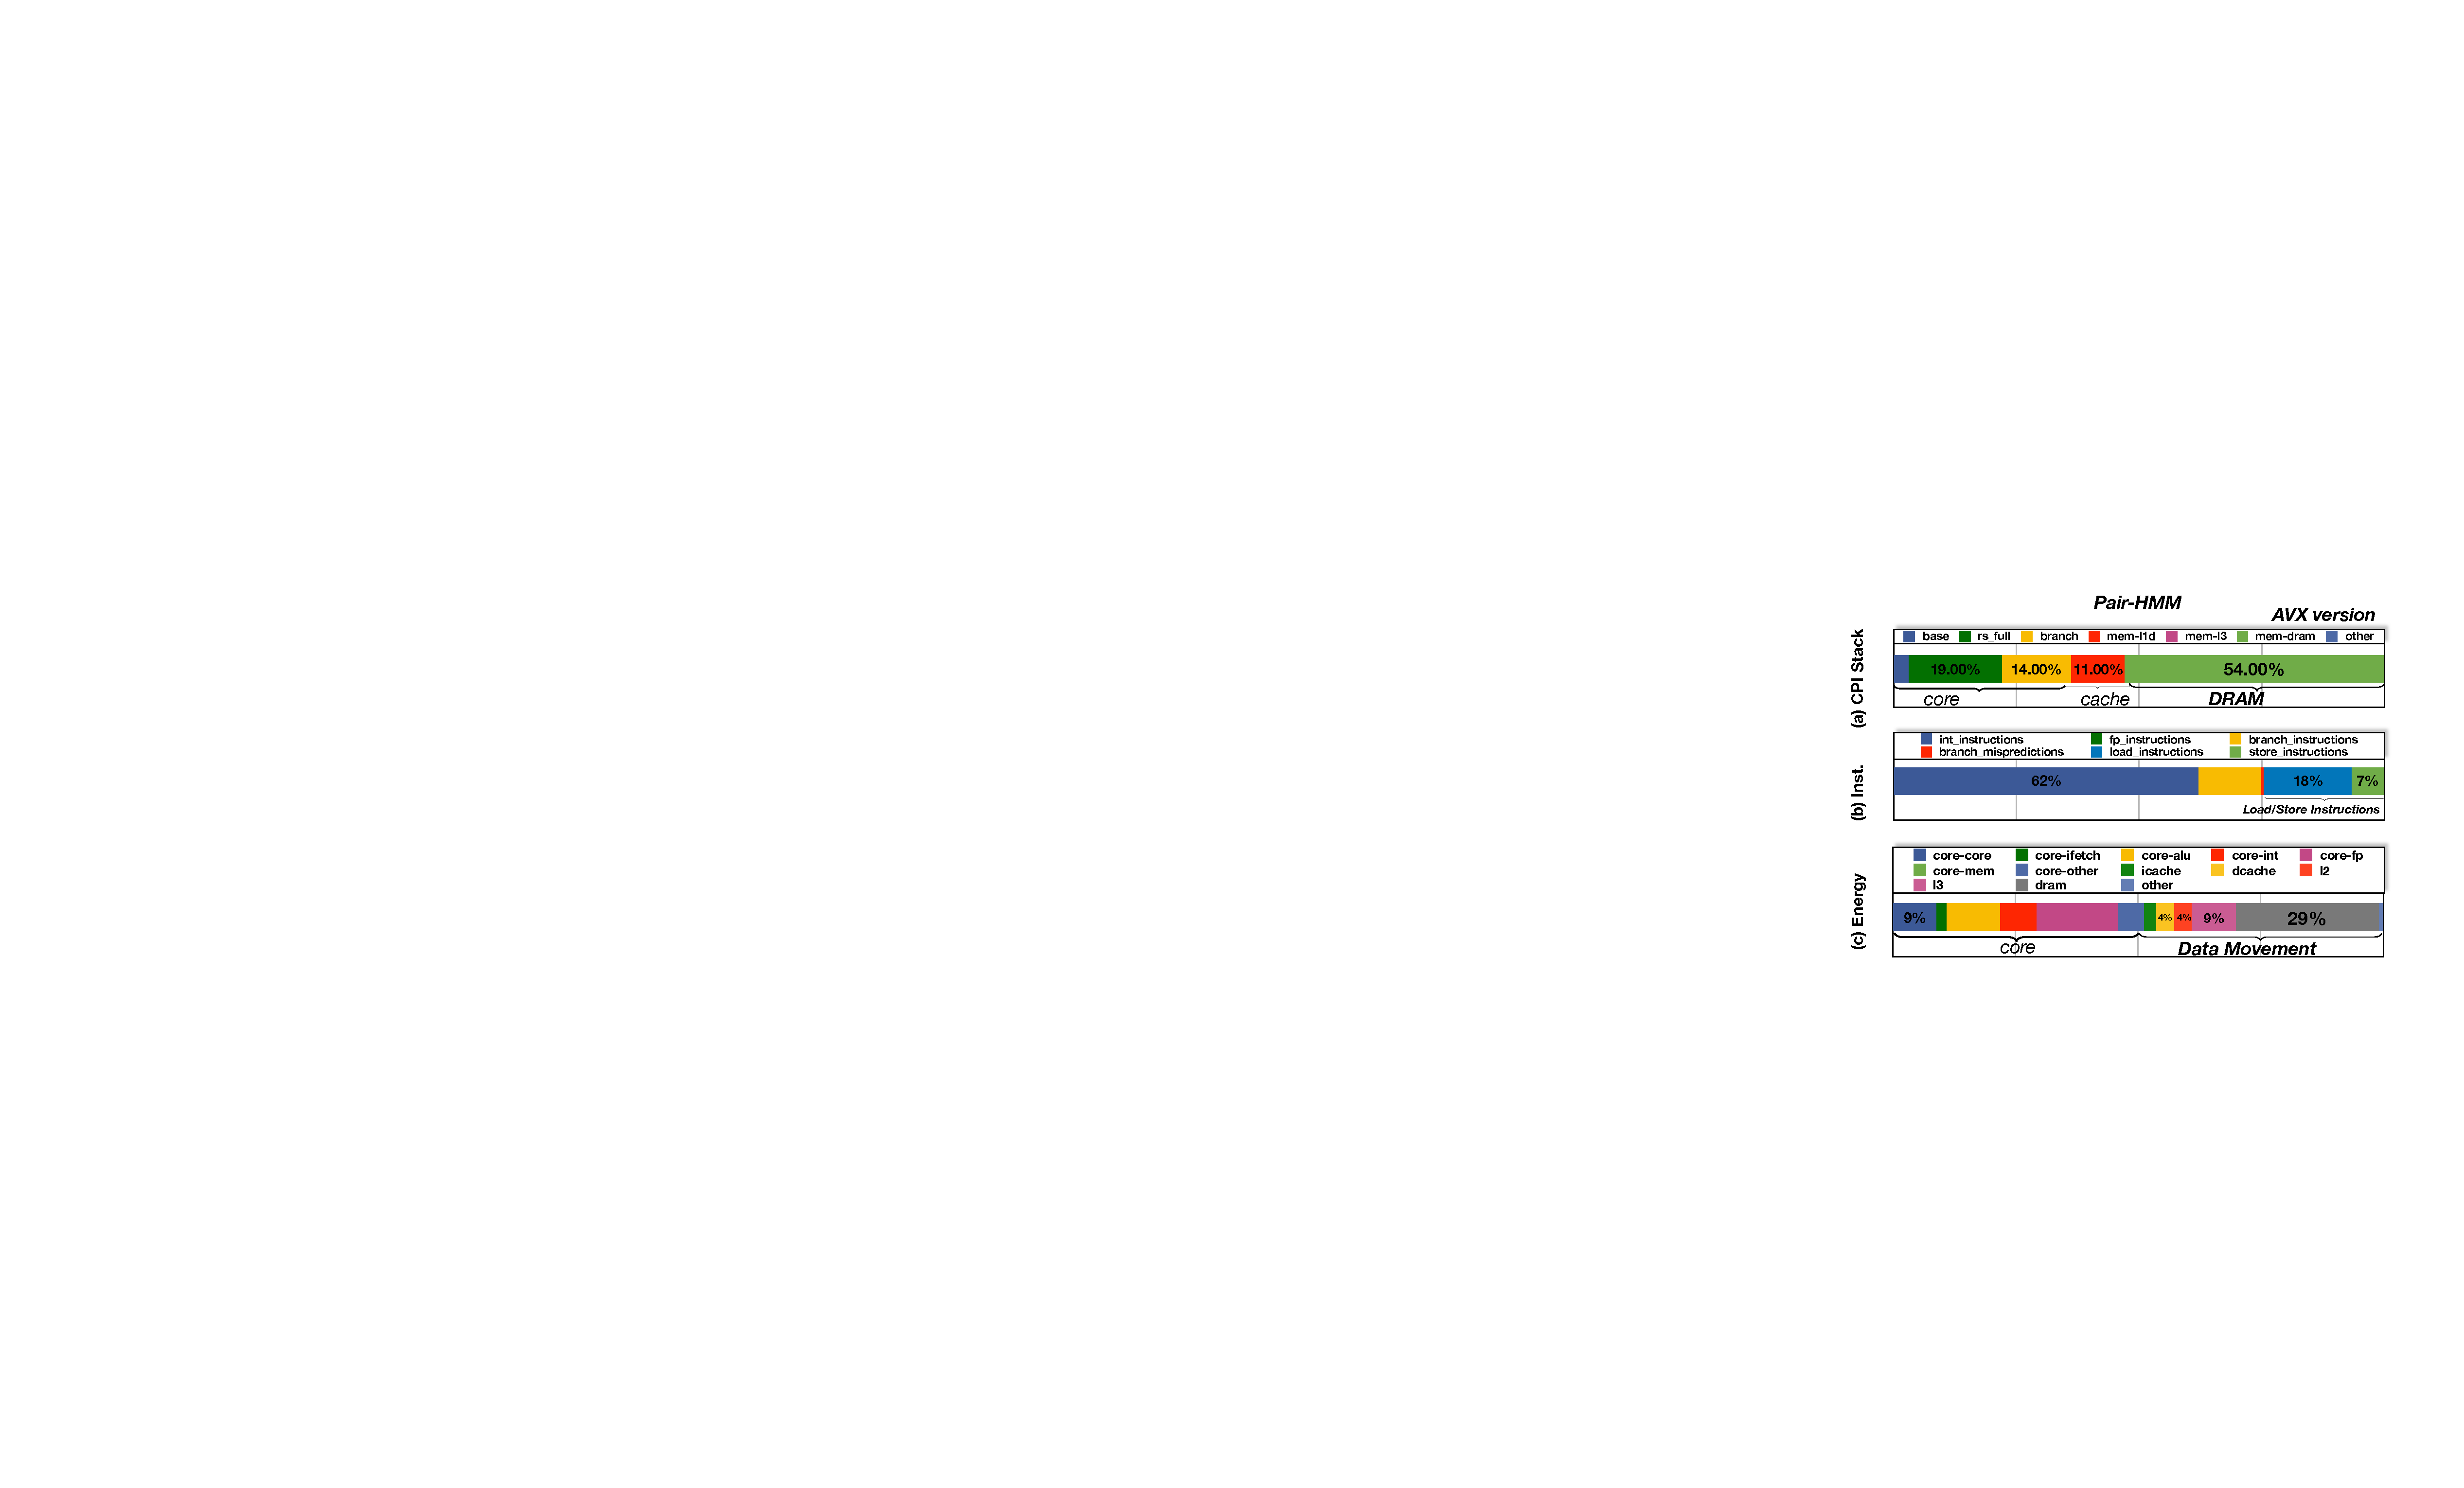
\includegraphics[scale=0.44]{fig/analysis/data-pair.pdf}
\caption{Profiling the Pair-HMM kernel with Sniper and configuration in Table II: (a) CPI stack; (b) Instruction statistics; (c) Energy breakdown.}
\label{fig:data-pair}
\end{figure}

\subsection{Key Insight From Data Movement Analysis}
Based on the analysis of the performance characteristics of these four typical kernels for genomic analysis, we observed that two of the four kernels FM-index based sequence search and Hash are memory-intensive. A significant fraction of data movement often comes from simple functions, e.g. memcopy, bitwise operations, and simple arithmetic operations. We can design lightweight logic to implement these simple functions in memory. FM-index and hash table suffer from irregular memory accesses and poor data locality. Although a software prefetch mechanism can reduce the problem to some extent. Prior work~\cite{yuanrong} revealed that only part of the prefetched cacheline can be utilized. The other two kernels -- Smith-Waterman and Pair-HMM -- are compute-intensive when they are ran with single thread. When considering multithreading mode, there is no guarantee that the data store will match all the calculated order, and the storage in a certain direction is not continuous, leading to a large number of TLB thrashing behaviors. It not make full use of the existing locality, in the column order calculation process, the same column of data may remain reused in the cache, the dependent row data is not reused. However, when calculating a column, a row or column size usually exceeds the cacheline size, The temporal locality of the cache mechanism makes the column data possibly in the cache, but the dependent row data needs to be read from the memory. Also, SW requires simple arithmetic operations to produce the result. PairHMM is the only kernel that uses floating point operations, and the floating operations limited to multiply and add. This class of compute-intensive operations does not have to be offloaded to PIMs, but we can offload them if there are idling hardware units in PIMs. In summary, we can report the following observations:

\begin{itemize}
    
    \item A significant fraction of data movement often comes from simple functions; we can design lightweight logic to implement these simple functions in memory. These operations are simple primitives: memcopy, bitwise operations, and simple arithmetic operations
    
    \item Genomic kernels have inherent intra- and inter-task parallelism to dig
    
    \item More bandwidth will help these kernels during the scaling process to achieve higher parallelism

\end{itemize}
